\documentclass{article}
\usepackage{graphicx}
\usepackage{float}

\graphicspath{ {images/} }

\newcommand{\projectnaam}{Software Reengineering}
\newcommand{\student}{Van Muylder Ben \& Geeraert Lander}
\title{\textmd{\textbf{Project Intermediate Report}}\\\normalsize\vspace{0.1in}\Large{\projectnaam}}
\author{\student}\date{\today}

\setcounter{section}{-1}

\begin{document}
\maketitle
\newpage

\section{Introduction}

For this intermediate report, we had to report upon the tools we will be using, have been using and have used to analyse how we want to refactor the project.\\

For each subsection, we provide a small explanation of which tools we may have used so far, or are planning to use, as well as a screenshot of those tools. 

\section{Tools Used}

First and foremost we want to mention that we often use Jetbrains IntelliJ and Codescene as starting points as they both provide functionality for multiple of the below mentioned subsections.

\subsection{Duplicate Code}

As an initial tool, we'll use IntelliJ (which provides simple assisting messages when it detects duplicate code) on the relevant parts of the code. Furthermore we'll use iClones to help us with further detection of duplicate code.

\begin{figure}[H]
\centering
	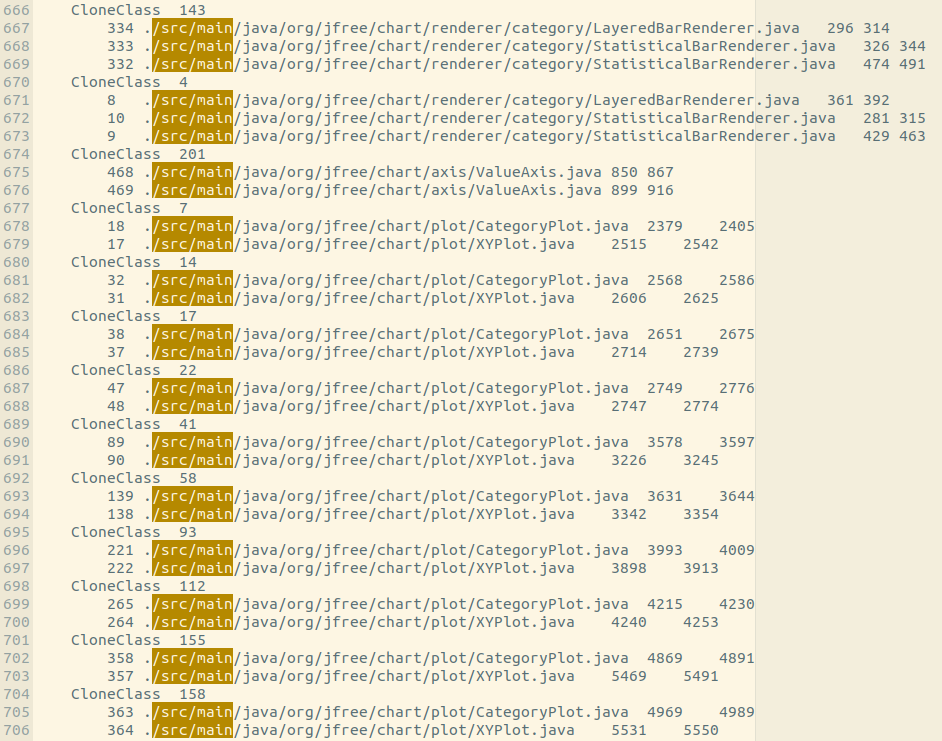
\includegraphics[width=0.9\textwidth]{iclones_dup.png}
	\caption{iClones Duplication Report}
\end{figure}

The duplication report showed us the presence of many duplications, mostly in the test classes, but some in the source classes as well. The question still remains how many of these duplications will actually be relevant for this assignment.

\subsection{Metrics and Visualisation}

For metrics and visualisation (as well as other things) we will mostly be using Codescene.

\begin{figure}[H]
\centering
	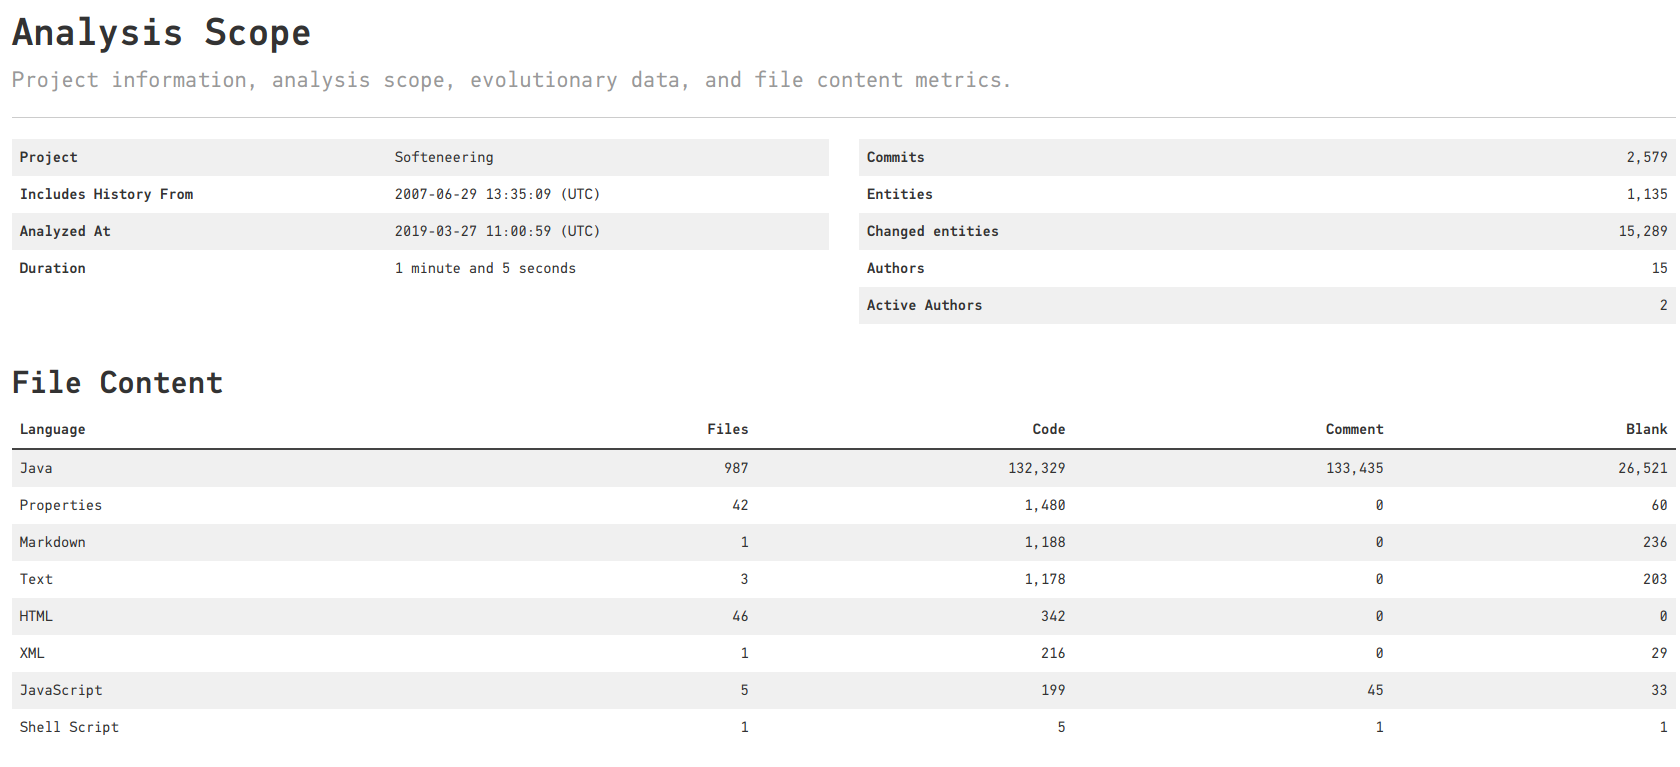
\includegraphics[width=0.9\textwidth]{codescene_analysis.png}
	\caption{Codescene Analysis}
\end{figure}


The link to our codescene project is given here as well, so  it can be used for further inspection. Note that the codescene project contains information about the project as we originally forked it from the original repository.\\

\noindent
https://codescene.io/projects/4473/jobs/12562/results

\newpage
\subsection{Mining Repositories}

We used Gsource, but as this mostly only provides a visual interactive history of your repository, this tool will be of no further use to us.\\

\noindent
We'll also use Codescene for this.


\begin{figure}[H]
\centering
	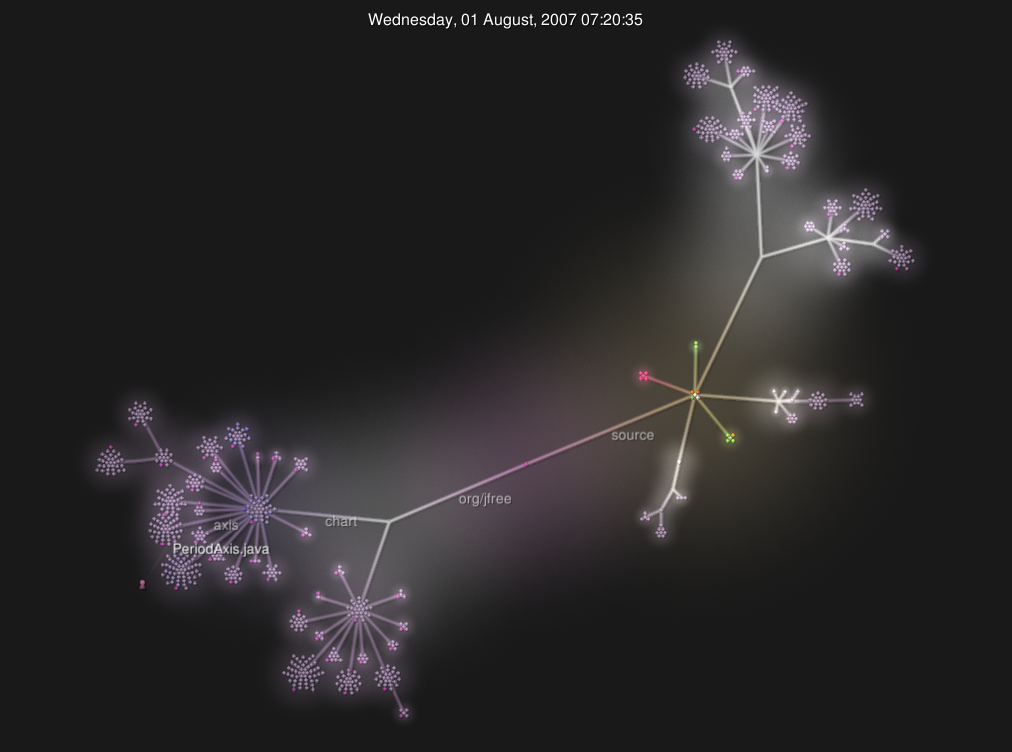
\includegraphics[width=0.9\textwidth]{gsource.png}
	\caption{Gsrouce in process}
\end{figure}

\newpage
\subsection{Refactoring Assistants}

As a baseline, we'll use IntelliJ to help us refactor (and specify what and how we should refactor) the project as well as Codescene which gives clear indications on what it thinks should be refactored. We will also have to lookup whether the assistance provided by codescene is relevant for our assignment.

\begin{figure}[H]
\centering
	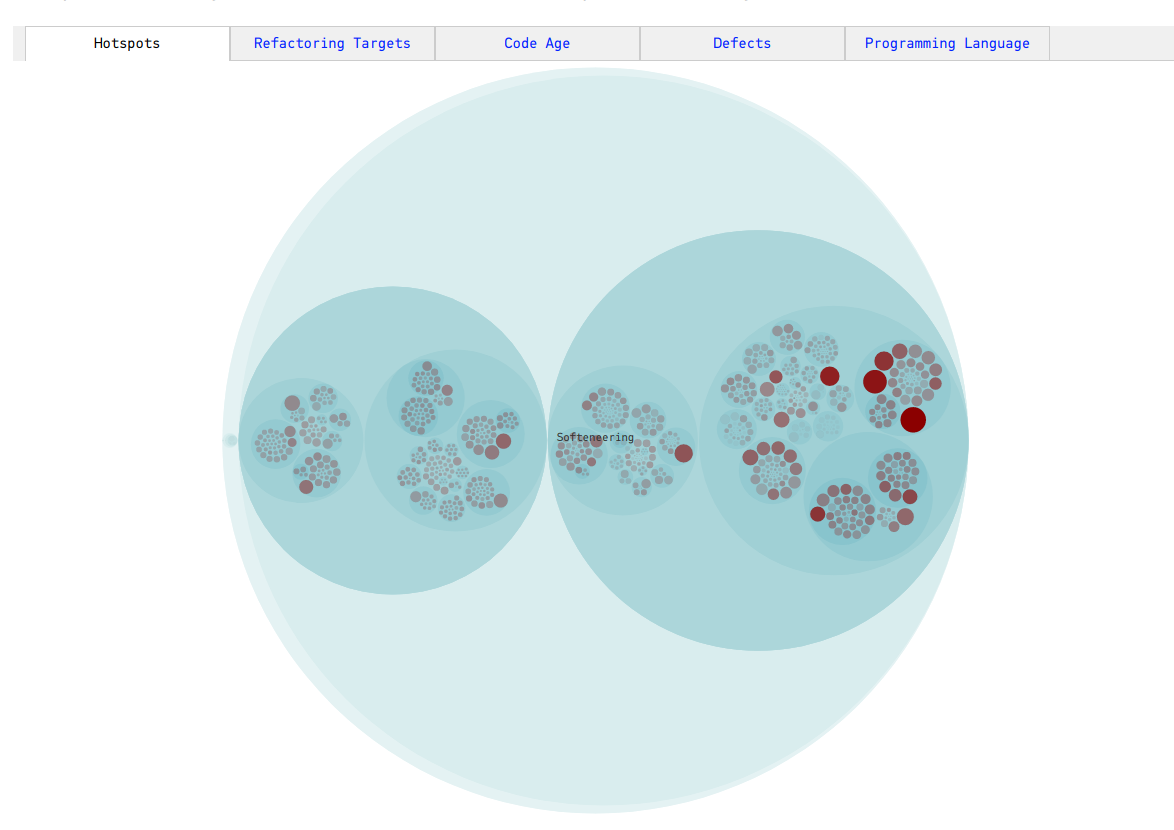
\includegraphics[width=0.9\textwidth]{codescene_hotspots.png}
	\caption{Codescene Hotspots}
\end{figure}

Here we can clearly see that both the classes XYPlot and CategoryPlot are highlighted as hotspots. This will most presumably be the classes most relevant for this assignment to refactor.

\newpage
\subsection{Test Coverage and Dynamic Analysis}

For test coverage, we plan on using LittleDarwin to perform mutation testing on the project. However, during our assignments for the Software Testing course, we already used LittleDarwin for that project, and even on such a small project it took a fairly long while to run LittleDarwin. Because of this, and because of the other tasks, assignments, etc. we had, we have not yet used LittleDarwin.\\

We also used cobertura (which was already present in the project) to get an initial overview of the test coverage.

\begin{figure}[H]
\centering
	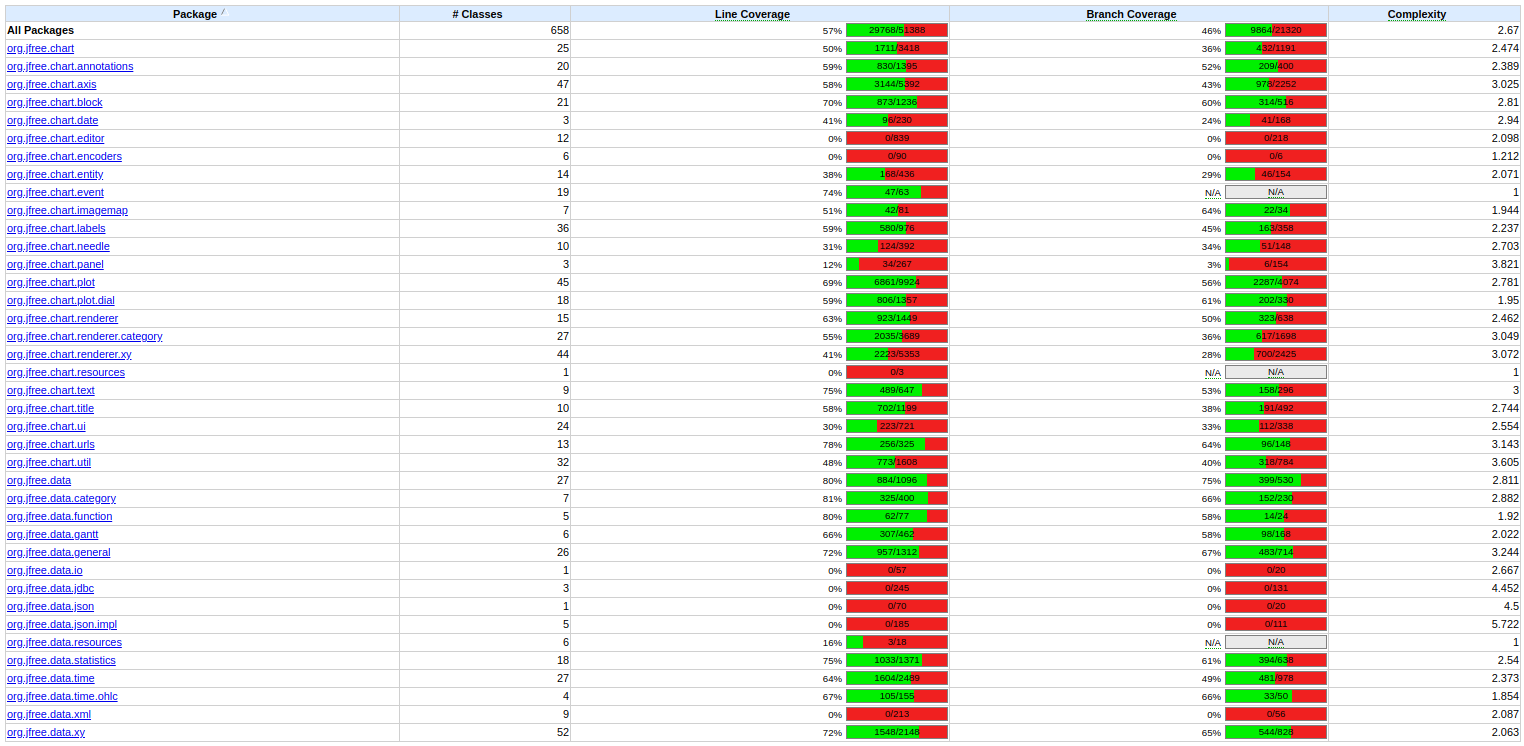
\includegraphics[width=0.9\textwidth]{cobertura_coverage.png}
	\caption{Cobertura Coverage Report}
\end{figure}

\subsection{Feature Location and Traceability}

Again, we will use IntelliJ as a baseline, but if it seems necessary, or if it seems that the functionality provided by IntelliJ is too limited, we'll look at other tools.\\

\noindent
(we provide no screenshot for this subsection)

\end{document}